%!TEX root = report.tex
\begin{figure}[h!]
\centering
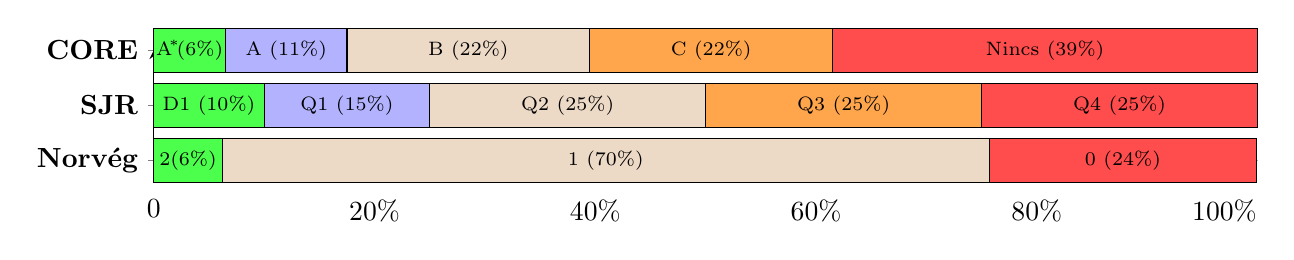
\begin{tikzpicture}
\begin{axis}[
    xbar stacked,
    xmin=0, xmax=100,
    width=156mm,
    height=3cm,
    bar width=16pt,
    enlarge y limits=0.3,
    y=7mm,
    symbolic y coords={Norvég,SJR,CORE},
    ytick=data,
    %xlabel={\%},
    xtick={0,20,40,60,80,97},
    xticklabels={0,20\%,40\%,60\%,80\%,100\%},
    axis x line=bottom,
    axis y line=left,
    yticklabel style={font=\bfseries},
    xticklabel style={
        yshift=-3mm,       % <-- itt tolod el 3mm-rel
        font=\normalsize  % ha nagyobbra akarod
    },
    nodes near coords,
    nodes near coords style={font=\scriptsize,inner sep=1pt,text=black},
    point meta=explicit symbolic,
    clip=false,
    draw=black
]

% ---- 1. szint: bal szélső szegmensek minden sorban ----
% Norvég: 2 (6.2%), SJR: D1 (10%), CORE: A* (7.4%)
\addplot+[xbar stacked, fill=green!70, font=\tiny, draw=black] coordinates {
  (6.2,Norvég) [2(6\%)]
  (10,SJR)     [D1 (10\%)]
  (6.5,CORE)   [A\!$^*$\!(6\%)] %all 84 found -> 7.5*.0.78
};
% ---- 2. szint ----
% Norvég: 1 (69.5%), SJR: Q1 (17%), CORE: A (12.5%)
\addplot+[xbar stacked, fill=blue!30, draw=black] coordinates {
  (0,Norvég) []
  (15,SJR)      [Q1 (15\%)]
  (11,CORE)   [A (11\%)] % 313 found 14 missing 13.8*0.78=10.76
};

% ---- 3. szint ----
% Norvég: 0 (24.2%), SJR: Q2 (25%), CORE: B (19.1%)
\addplot+[xbar stacked, draw=black] coordinates {
  (69.5,Norvég) [1 (70\%)]
  (25,SJR)      [Q2 (25\%)]
  (22,CORE)   [B (22\%)] % 17.7% + 2.3% A* short  434 found 177 missing -> 614 total -> 30% hiányzik (8%-a a teljesnek) 28.3*0.78
};

% ---- 4. szint ----
% Norvég: nincs további kategória (0), SJR: Q3 (25%), CORE: C (20.6%)
\addplot+[xbar stacked,  fill=orange!70, draw=black] coordinates {
  (0,Norvég)    []
  (25,SJR)      [Q3 (25\%)]
  (22,CORE)   [C (22\%)] % 10.9% + 2.9% A short 516 found + 517 missing (50% hiányzik, ami 14%-a a teljesnek) 27.6*0.78
};

% ---- 5. szint ----
% Norvég: 0, SJR: Q4 (25%), CORE: Nincs (40.4%)
\addplot+[xbar stacked,  fill=red!70, draw=black] coordinates {
  (24.2,Norvég)    [0 (24\%)]
  (25,SJR)      [Q4 (25\%)]
  (38.5,CORE)   [Nincs (39\%)] %(azaz 22%-kal több cikk lehet.)
};

\end{axis}
\end{tikzpicture}

\caption{A Norvég, SJR és CORE értékelések kategória-határai 0--100\% skálán.}
\label{fig:core_boundaries}    
\end{figure}